%template1.tex
%The following LaTeX source file represents the simplest kind of slide presentation; no overlays, no included graphics. Substitute your favorite style for ``pascal''. To create the PDF file template1.pdf, (1) be sure to use the prosper class, then (2) execute the command latex template1.tex, and (3) the command dvipdf template1.dvi.

%%%%%%%%%%%%%%%%%%%%%%%%%%%%%%% template1.tex %%%%%%%%%%%%%%%%%%%%%%%%%%%%%%%%%%%
\documentclass[a4paper,blends,pdf,colorBG,slideColor]{prosper}
% definitions for slides for CSC544
% Lutz Hamel, (c) 2007

\hypersetup{pdfpagemode=FullScreen}

\usepackage{times}
\usepackage{latexsym}
\usepackage{alltt}
\usepackage{booktabs}
\usepackage{amsmath}
\usepackage{amsopn}
\usepackage{amsfonts}
\usepackage{amssymb}
%\usepackage[usenames]{color}

\def\sign{\qopname\relax{no}{sign}}
\def\argmax{\qopname\relax{no}{argmax}}
\def\argmin{\qopname\relax{no}{argmin}}

\newcommand{\grad}{\ensuremath{\nabla}} 
\newcommand{\loss}{\ensuremath{{\cal L}}}
\newcommand{\err}{\mbox{err}}
\newcommand{\mse}{\mbox{mse}}
\newcommand{\acc}{\mbox{acc}}
\newcommand{\Integer}{\ensuremath{\mathbb{N}}}
\newcommand{\size}[1]{{|{#1}|}}
\newcommand{\Rnspace}[1]{\ensuremath{\mathbb{R}^{#1}}}
\newcommand{\Real}{\ensuremath{\mathbb{R}}}
\newcommand{\mytt}[1]{{\small\tt{#1}}}
\newcommand{\textemph}[1]{{\em #1}}
\newcommand{\suchthat}{\mid}
\newcommand{\orbar}{\;|\;}
\newcommand{\bs}[1]{\begin{slide}{#1}\ptsize{8}}
\newcommand{\es}{\end{slide}}
\newcommand{\co}{\,\colon\;}
\newcommand{\pair}[2]{\ensuremath{( {#1}, {#2} )}}
\newcommand{\model}[1]{\hat{#1}}
\newcommand{\ul}[1]{{\bf\em #1}}
\newcommand{\ol}{\overline}
\newcommand{\definition}[1]{{\bf Definition: }{\em #1}}
\newcommand{\example}[1]{{\bf Example: }{#1}}
\newcommand{\abs}[1]{|{#1}|}
\newcommand{\mytab}{\makebox[.1in]{}}

\newcommand{\fdef}[1]{
\begin{center}
\fbox{
\begin{minipage}{3.5in}
{\bf Definition:}
{#1}
\end{minipage}
}
\end{center}
}

\newcommand{\fframe}[1]{
\begin{center}
\fbox{
\begin{minipage}{3.5in}
{#1}
\end{minipage}
}
\end{center}
}

\newcommand{\nframe}[1]{
\begin{center}
\begin{minipage}{3.5in}
{#1}
\end{minipage}
\end{center}
}

\newenvironment{Rcode}
	{
		\scriptsize
		\begin{quote}
		\begin{alltt}
	}
	{
		\end{alltt}
		\end{quote}
	}




\begin{document}

\bs{Duality}
Duality is a powerful algorithm design tool that allows us to explore different algorithmic alternatives
based on the inherent constraints of the underlying problem.  

In our case the constraints on the solution (the position of the decision surface) are the observations
close to the class boundaries where the classes meet.

We find that the dual solution is dominated by the constraints represented by the points close to the class boundaries.
\es

\bs{Perceptron Learning}
\begin{center}
\begin{minipage}{3in}
{\small
$\vdots$\\
{\bf repeat}\\
\mytab {\bf for} $i = 1$ {\bf to} $l$\\
\mytab\mytab {\bf  if} {\color{red}$\sign(\ol{w}\bullet\ol{x}_i - b) \neq y_i$} {\bf then}\\
{\color{red}\mytab\mytab\mytab $\ol{w} \leftarrow \ol{w} + \eta y_i \ol{x}_i$}\\
\mytab\mytab\mytab $b \leftarrow b - \eta y_i r^2$\\
\mytab\mytab {\bf end if}\\
\mytab {\bf end for}\\
{\bf until} $\sign(\ol{w}\bullet\ol{x}_j - b) = y_j$ {\rm with} $j = 1,\ldots,l$\\
$\vdots$
}
\end{minipage}
\end{center}

\vspace{.2in}
{\bf Observation:}  $\ol{w}$ will contain many copies of the scaled position vector $\ol{x}_i$ for ``difficult'' points;  points that are difficult to classify.

{\bf Idea:} Instead of updating the normal vector of the decision surface, count the number
of times a particular point is being misclassified.

\es

\bs{Duality}
Introduce a new variable that keeps track of the misclassification counts:
\[
\ol{\alpha} = (\alpha_1, \ldots,\alpha_l)
\]
Then we can write our learning algorithm as,

\begin{center}
\fbox{
\begin{minipage}{2in}
{\small
Initialize $\ol{\alpha}$ and $b$ to 0.\\
{\bf repeat}\\
\mytab {\bf for each} $(\ol{x}_i,y_i) \in D$ {\bf do}\\
\mytab\mytab {\bf  if} {\color{red}$\model{f}(\ol{x}_i) \ne y_i$} {\bf then}\\
\mytab\mytab\mytab {\color{red}Increment $\alpha_i$ by $1$}\\
\mytab\mytab\mytab Update $b$\\
\mytab\mytab {\bf end if}\\
\mytab {\bf end for}\\
{\bf until} $D$ is perfectly classified\\
{\bf return} $\ol{\alpha}$ and $b$
}
\end{minipage}
}
\end{center}
{\bf Problem:} How do we represent our free parameter $\ol{w}$ using $\ol{\alpha}$? Or $\model{f}$
for that matter?
\es


\bs{Duality}
\begin{center}
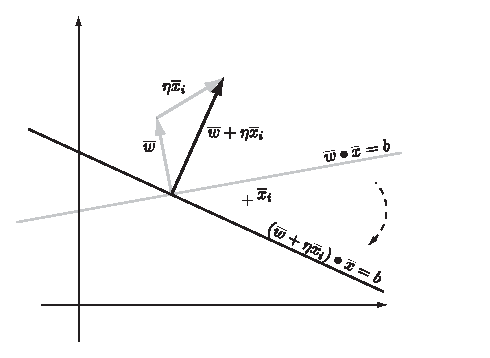
\includegraphics[height=40mm]{figures/fig05-02.eps}
\end{center}

\begin{align*}
\ol{w} &= \sum_{i=1}^l \eta\alpha_i y_i \ol{x}_i\\
	 &= \eta \sum_{i=1}^l \alpha_i y_i \ol{x}_i.
\end{align*}

\es

\bs{Duality}
This means that we can rewrite
the normal vector $\ol{w}$ as the following sum,
\begin{align*}
\ol{w} &= \sum_{i=1}^l \alpha_i y_i \ol{x}_i\\
\intertext{ where }\\
\alpha_i &\approx 0 \mbox{ for ``easy'' points,}\\
\alpha_i &\gg 1 \mbox{ for ``difficult'' points.}
\end{align*}

{\bf Note:} The learning rate $\eta$ is simply a scaling constant of the resulting 
normal vector $\ol{w}$ and since we are primarily interested in the orientation of the decision 
surface it is customary to drop this constant.
\es

\bs{Duality}
Now our perceptron decision function now looks like
\begin{align*}
\model{f}(\ol{x}) &= \sign(\ol{w}\bullet\ol{x} - b)\\
&= \sign\left((\sum_{i=1}^l \alpha_i y_i \ol{x}_i\bullet\ol{x}) - b\right)
\end{align*}
where $l$ is the number of instances in $D$.
\es

\bs{Duality}
\begin{center}
\fbox{
\begin{minipage}{3in}
{\small
{\bf let} $D = \{(\ol{x}_1,y_1), (\ol{x}_2,y_2),\dots,(\ol{x}_l,y_)\} \subset \Rnspace{n} \times \{+1, -1\}$\\
{\bf let} $0 < \eta <1$\\
$\ol{\alpha} \leftarrow \ol{0}$\\
$b \leftarrow 0$\\
$r \leftarrow \max \{ \abs{\ol{x}} \mid (\ol{x},y)\in D\}$\\
{\bf repeat}\\
\mytab {\bf for} $i = 1$ {\bf to} $l$\\
\mytab\mytab {\bf if} {\color{red}$\sign(\sum_{j=1}^l \alpha_j y_j \ol{x}_j\bullet\ol{x}_i - b) \neq y_i$ }{\bf then}\\
\mytab\mytab\mytab {\color{red}$\alpha_i \leftarrow \alpha_i + 1$}\\
\mytab\mytab\mytab $b \leftarrow b - \eta y_i r^2$\\
\mytab\mytab {\bf end if}\\
\mytab {\bf end for}\\
{\bf until} $\sign(\sum_{j=1}^l \alpha_j y_j \ol{x}_j\bullet\ol{x}_k - b) = y_l$ {\rm with} $k = 1,\ldots,l$\\
{\bf return} $(\ol{\alpha}, b)$
}
\end{minipage}
}
\end{center}
\es


\bs{Duality}
The two perceptron learning algorithms give rise to different representations
of the induced decision surface.

\vspace{.5in}

\begin{center}
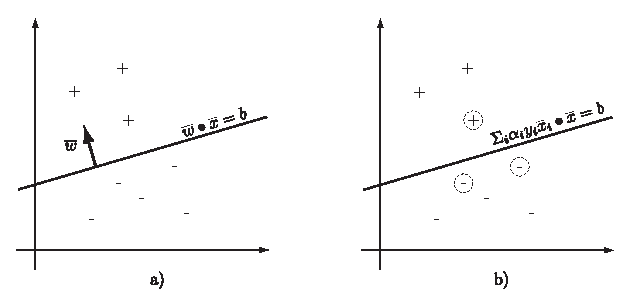
\includegraphics[height=40mm]{figures/fig05-05.eps}
 \end{center}
 \es
 
\bs{Duality}
The dual algorithm still can give rise to degenerate decision surfaces.

\vspace{.5in}

\begin{center}
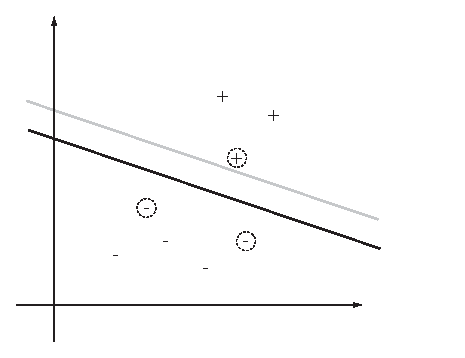
\includegraphics[height=40mm]{figures/fig05-06.eps}
 \end{center}

\es
\end{document}
%%%%%%%%%%%%%%%%%%%%%%%%%%% end of template1.tex %%%%%%%%%%%%%%%%%%%%%%%%%%%%%%%%

